\documentclass[12pt,letterpaper,noanswers]{exam}
\usepackage[usenames,dvipsnames,svgnames,table]{xcolor}
\usepackage[margin=0.9in]{geometry}
\renewcommand{\familydefault}{\sfdefault}
\usepackage{multicol}
\pagestyle{head}
\header{AM 108 Class 09}{}{2d Systems (page \thepage)}
\runningheadrule
\headrule

\usepackage{graphicx} % more modern
\usepackage{amsmath} 
\usepackage{amssymb} 

\usepackage{hyperref}
\usepackage{tcolorbox}

\begin{document}
 \pdfpageheight 11in 
  \pdfpagewidth 8.5in

\noindent 





\begin{itemize}
\itemsep0em
    \item There is a problem set due on Friday.
   % \item Problem Set 02 will be due this Friday.
    \item There is a two question skill check on Friday.  The question info is below.
    \item Find office hours info on the Canvas page.
    \item Our first quiz will be on Monday Sept 28th (there is no class meeting that day).  There is info on Canvas.  The quiz will be via Gradescope.
    \item There is a discussion board post summary assignment due on Friday.  It is on Canvas (and is not long).
\end{itemize}

\hrule
\vspace{0.2cm}


\noindent\textbf{Teams}

\begin{multicols}{2}
1. 
\end{multicols}

\noindent \textbf{Teams 3 and 4}: Post screenshots of your work to the course Google Drive today.  Include words, labels, and other short notes that might make those solutions useful to you or your classmates.  Find the link in Canvas (or here: \url{https://drive.google.com/drive/u/0/folders/1GcpwvKHD4tMecpFQ4lNxN_r5Ylj7YHbd})


\vspace{0.2cm}
\hrule
\vspace{0.2cm}


\noindent \textbf{Extra vocabulary / extra facts:}
\begin{tcolorbox}

Given solutions, $x = a$ and $x = b$, to a quadratic equation, we can construct such an equation: $(x-a)(x-b) = 0$.  Other quadratic equations with these solutions would be multiples of this equation.

If two polynomial equations, with coefficients $a_0, a_1, ..., a_n$ and $b_1, b_2, ..., b_n$, have the identical solutions, then their coefficients are equal up to a constant: $a_0 = c b_0, a_1 = c b_1, ... a_n = c b_n$.
\end{tcolorbox}

\vspace{0.2cm}
\hrule
\vspace{0.2cm}
\noindent{From Monday}

\begin{questions}
\item (Generic 2d system of linear differential equations) 

Consider the system 
\begin{align*}
\frac{dx}{dt} =&\ ax + by \\
\frac{dy}{dt} =&\ cx + dy
\end{align*}
with fixed point at the origin.
\begin{parts}
\item Rewrite this in matrix / vector form (let $\displaystyle \underline{x} = \left(\begin{array}{c} x \\ y \end{array}\right).)$
\item Let $\displaystyle A = \left(\begin{array}{c c} a & b \\ c & d \end{array}\right).$  Recall that the eigenvalues of $A$, $\lambda_1$ and $\lambda_2$, are given by $\lambda^2 - \tau \lambda + \Delta = 0$ where $\tau = a +d $ is the trace of the matrix $A$ and $\Delta = ad - bc$ is the determinant of the matrix $A$.  In addition, $(\lambda - \lambda_1)(\lambda-\lambda_2) = 0$.  Why?
\item Use this second fact (and match terms in the two equations) to show that $\lambda_1 + \lambda_2 = \tau$ and $\lambda_1\lambda_2 = \Delta$.
\item Consider the $\Delta\tau$-plane (with $\Delta$ on the horizontal axis).  Identify regions of the $\Delta\tau$ plane where the matrix has two negative eigenvalues, regions where it has one positive eigenvalue and one negative one, and regions where it has two positive eigenvalues.
\item Consider $\underline{v}e^{\lambda_1 t}$, where $\lambda_1$ is an eigenvalue of $A$ and $\underline{v}$ is the associated eigenvector.  Show that this is a solution of the differential equation (Steve did this in the linear systems video, and it's fine to follow his steps).  Think about plotting this solution as a trajectory in the $xy$-plane.  Why is it a straight-line solution?
\item General solutions to this differential equation are of the form $\displaystyle\underline{x}(t) = c_1\underline{v}_1e^{\lambda_1 t} + c_2\underline{v}_2e^{\lambda_2 t}$.  We might have $\lambda_1$ and $\lambda_2$ both real.  Or they could be a complex conjugate pair, where $\lambda_1 = \lambda+i\omega$ and $\lambda_2 = \lambda-i\omega$.  When they are a complex conjugate pair, we require the solution to the differential equation to be real, so we require $c_1$ and $c_2$ to be a complex conjugate pair as well.

For the systems
\[ 
\begin{array}{ r l c r l c r l c r l c}
 \dot{x} =  &x  & \quad & \dot{x} = &-x - y & \quad & \dot{x} = &\ x & \quad & \dot{x} =&\ x + y \\
 \dot{y} = &x- y & \quad & \dot{y} = &\ x - 2y & \quad & \dot{y} = &- y & & \dot{y} = &-2x + y\\
\end{array}\]
find their trace and their determinant.  Which have real eigenvalues and which have eigenvalues that are a complex conjugate pair?

\item Attempt to match the systems above to the phase portraits below.

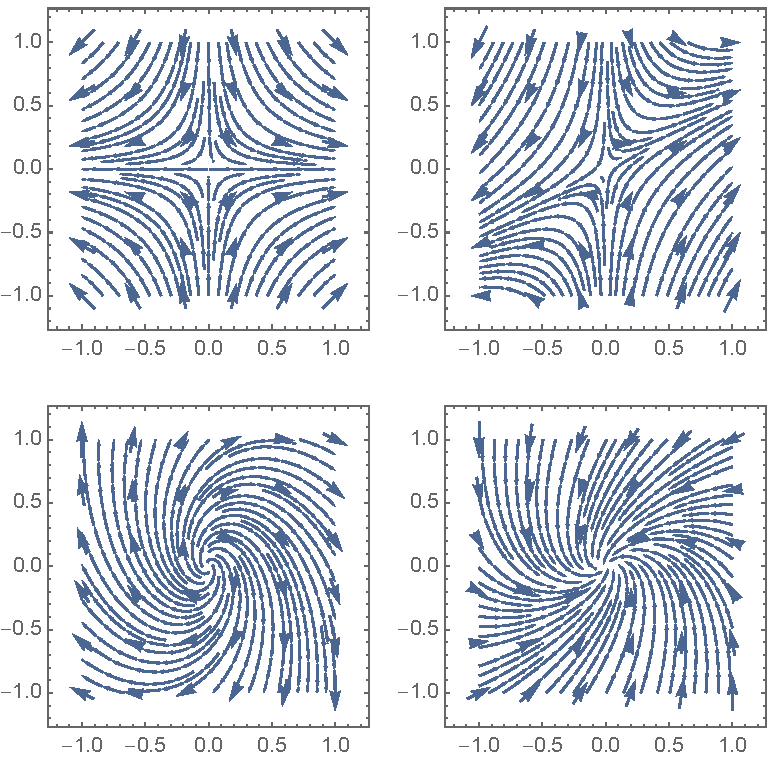
\includegraphics[width=5in]{img/VectorFields.pdf}
\end{parts}
\end{questions}


\vspace{0.2cm}
\hrule
\vspace{0.2cm}


\noindent \textbf{Extra vocabulary / extra facts part 2:}

\begin{tcolorbox}
The \textbf{Hartman-Grobman} theorem tells us when we can use a linear system to approximate the behavior of a nonlinear system near a fixed point.  

\textbf{Hartman-Grobman} theorem: When the fixed point is hyperbolic and the vector field is continuously differentiable (called $C^1$ where $1$ indicates the 1st derivative is continuous), there is a neighborhood of the fixed point where the linearization is a good approximation that preserves the stability properties of the fixed point.

For a vector-valued function of several variables, $\mathbf{f}(\mathbf{x})$, the \textbf{Jacobian matrix} is a matrix of first order partial derivatives,
\[\left(\begin{array}{c c c} \frac{\partial f_1}{\partial x_1} & \cdots & \frac{\partial f_1}{\partial x_m} \\ \vdots & \ddots & \vdots \\
\frac{\partial f_n}{\partial x_1} & \cdots & \frac{\partial f_n}{\partial x_m}
\end{array}\right)\]
and is sometimes denoted $D\mathbf{f}$.

The term \textbf{Jacobian} refers either to a square Jacobian matrix (when there are $n$ equations and $n$ variables), or to the determinant of that matrix.

\end{tcolorbox}

\textbf{Borderline} cases:

Steve emphasizes that in between nodes and spirals there is a borderline case.  We won't really treat that as a borderline case, however.  

We will reserve 'borderline' for non-hyperbolic cases.  These are places where the real part of one of the eigenvalues is zero.  The borderline cases correspond to a change in fixed point from attractor to repeller (linear center), from attractor to saddle (line of attracting fixed points) or from repeller to saddle (line of repelling fixed points).

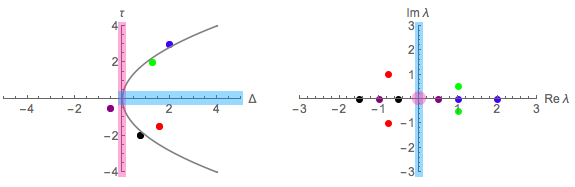
\includegraphics[width=\linewidth]{img/S19Week07p2.png}

\vspace{0.2cm}
\hrule
\vspace{0.2cm}

\noindent\textbf{Addressing your questions}

\begin{enumerate}
\itemsep0em
    \item For a degenerate node, where  a solution $\underline{x}(t)$ is given by $\underline x(t) = c_1 \underline{v}e^{\lambda t} + c_2(\underline{v} t + \underline{u})e^{\lambda t}$, how does this result in the phase portrait that we see?


In blue is the vector field for $0<\tau^2-4\Delta \ll 1$ and in orange for $1 \ll \tau^2-4\Delta < 0$.  

On the left these are on either side of a degenerate node.  On the right these are on either side of a star node.

Black lines are eigenvectors.

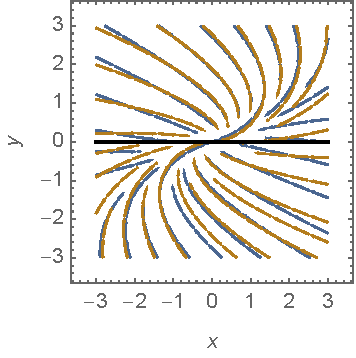
\includegraphics[]{img/C08spiral-vs-nodep1.pdf}
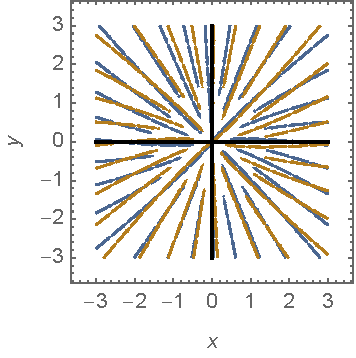
\includegraphics[]{img/C08spiral-vs-nodep2.pdf}

\item For repelling nodes, do trajectories move in parallel with the slow direction or the fast one as $t \rightarrow \infty$?

See {\color{blue}  \href{https://harvard.zoom.us/rec/play/lX1ny4yNnMY6JJHgyRA7oOCTstSUGg_nz8JoeiFCVCyR54jITe-WA-D0mhz-z3fkm7QOWwXl53OYOm1Q.rRkoIFXuq3kkTMa1}{minute 37:30 from C08}} for reasoning about attracting nodes.  

\end{enumerate}
\vspace{0.2cm}

\hrule
\vspace{0.2cm}

\noindent\textbf{Skill Check C10 practice}
\begin{questions}

\item Retake of Skill Check C07 on the time evolution of a phase difference.  See the C06 handout for the sample question.

\item Use $\tau$ and $\Delta$ to provide classifications for the following linear systems.  
\begin{parts}
\item Classify each fixed point as either stable (attractors), unstable (repellers or saddle points), or non-hyperbolic (a line or plane of fixed points, or a center). 
\item Identify the type of fixed point(s) (attractor, repeller, saddle point, linear center, line of fixed points, plane of fixed points).  Also specify spiral vs node, if relevant.
\end{parts} 

\begin{tabular}{|c|c|c|c|}
\hline
$\tau$ & $\Delta$ & stable / & attractor, etc/ \\
& & unstable / &  \\
& & non-hyperbolic & \\
\hline
2 & 3 & & \\
&  & & \\
\hline
 1    &  -2& & \\
     & & & \\
     \hline
 0  & 3 & & \\
     & & & \\
     \hline
\end{tabular}
\end{questions}

\vspace{0.2cm}

\hrule
\vspace{0.2cm}

\noindent\textbf{Skill Check C10 practice solution}

2. 
\begin{itemize}
    \item $\tau = 2$, $\Delta = 3$.  $\Delta > 0$ so this is not a saddle point.  $\tau > 0$, so this is a repeller (unstable).  $\tau^2 - 4\Delta = 4 - 12 = -8<0$, so this is a spiral.
    \item $\tau = 1, \Delta = -2$.  $\Delta < 0$ so this is a saddle point, which is an unstable fixed point.
    \item $\tau = 0$, $\Delta = 3$.  $\Delta > 0$ so not a saddle point.  $\tau = 0$ so this is a linear center.  non-hyperbolic (real part of each eigenvalue is zero).
\end{itemize}


\begin{tabular}{|c|c|c|c|}
\hline
$\tau$ & $\Delta$ & stable / & attractor, etc/ \\
& & unstable / &  \\
& & non-hyperbolic & \\
\hline
2 & 3 & unstable & repeller (spiral) \\
&  & & \\
\hline
 1    &  -2& unstable & saddle point\\
     & & & \\
     \hline
 0  & 3 & non-hyperbolic & linear center\\
     & & & \\
     \hline
\end{tabular}



\vspace{0.2cm}

\hrule
\vspace{0.2cm}

\begin{questions}
\setcounter{question}{1}
\item (6.3.6) Consider the system
$\displaystyle\begin{array}{c c c}
 \dot{x} = & f(x,y) = x y - 1 \\
 \dot{y} = & g(x,y) = x - y^3
\end{array}$
 \begin{parts}
 \item Use \textbf{substitution} to show that $(-1,-1)$ and $(1,1)$ are both fixed points of the system (i.e. is $f(x,y) = 0$ and $g(x,y) = 0$ at these points?).  
 
 Determine whether there are other fixed points.
 \item Use Taylor polynomials to approximate the dynamical system to second order about the fixed point $(-1, -1)$.  
 
 Let $u = x-(-1)$, $v = y - (-1)$ and use this to simplify your expressions.
 
 \emph{I am asking you to approximate to second order as a review of Taylor approximation.}
 
 \begin{tcolorbox}
 
 Extra notes on Taylor polynomials:
 
 When we find a linear approximation (a first order Taylor polynomial) to a function at a point $Q$ we are identifying a linear function that has the same value as the function of interest at $Q$ and that has the same first derivatives as the original function at $Q$.
 
 When we construct a higher order approximation, of order $p$  (a $p$th order Taylor polynomial), we are finding a function such that the first $p$ derivatives match between the approximation and the original function at $Q$.
 
It may be helpful to recall that
 \begin{align*} 
 f(x,y) \approx& f(a,b) + (x-a)f_x(a,b) + (y-b) f_y(a,b) + (x-a)^2\frac{f_{xx}(a,b)}{2}\\
 &+(x-a)(y-b)f_{xy}(a,b) + (y-b)^2\frac{f_{yy}(a,b)}{2} + h.o.t.
 \end{align*}

\end{tcolorbox}
\item Sufficiently close to $(-1,-1)$, we have $\vert u \vert, \vert v\vert \ll 1$ and $u^2 \ll \vert u \vert, v^2 \ll \vert v \vert,$ so quadratic order and higher terms are small relative to the linear terms.  

\emph{Notation note: $\ll$ is read as `much less than'.  If you'd like to read a discussion of its meaning, see}

\small{\url{https://math.stackexchange.com/questions/1516976/much-less-than-what-does-that-mean#1516998}}
\begin{itemize}
\item Drop these higher order terms to generate a linearization of the system.  
\item Use your linearization to write a dynamical system of the form \[\dot{\underline{u}} = A \underline{u},\] giving definitions for $\underline{u}, A$. \\
\item Explain why the linearization leads to this kind of matrix equation only at a fixed point.  What would be the form of the linearized system away from a fixed point?
\end{itemize}

\item Create a linearized system about the fixed point $(1,1)$ as well.
\item Classify your fixed points as  \textbf{hyperbolic} (\emph{no eigenvalues have zero real part}) or \textbf{nonhyperbolic} 
 (\emph{at least one eigenvalue has zero real part}) fixed points.  \\ 
 
 \emph{Since $\Delta = \lambda_1\lambda_2$, there is a zero eigenvalue when $\Delta = 0$.  If $\tau = 0$ there may be a complex conjugate pair of eigenvalues with zero real part, the eigenvalues might both be real and sum to zero, or the eigenvalues might both be zero.  In the case of a c.c. pair with zero real part, find the sign of the determinant.} \\
 
The Hartman-Grobman theorem tells us that stability information from the linearization can be used to classify hyperbolic fixed points.  When a fixed point is nonhyperbolic the stability information from linearization is not so useful.
 \\

Identify the stability of any hyperbolic fixed points.  (Classify them as attracting, repelling, or saddle points, and identify whether they are stable or unstable).
 
  \item Use eigenvalues and eigenvectors to sketch neighboring trajectories to the two fixed points.  Try to fill in the rest of the phase portrait.  \\
  
  What do you think the long term behavior would be for a trajectory starting at $(2,2)$?  What about for one starting at $(1,2)$?

 \end{parts}

\end{questions}

\eject


%For what conditions on $\lambda_1$ and $\lambda_2$ (and thus on $\tau$ and $\Delta$) would all solutions eventually approach the fixed point at $\underline{x} = \underline{0}$?

\eject 
\textbf{Answers:}
\begin{questions}
    \item \begin{parts}
    \item $\displaystyle \underline{x} = \left(\begin{array}{c} x \\ y \end{array}\right)$, $\displaystyle \dot{\underline{x}} = \frac{d}{dt}\left(\begin{array}{c} x \\ y \end{array}\right),$ $A = \left(\begin{array}{c c} a & b \\ c & d \end{array}\right)$.  The equation becomes $\dot{\underline{x}} = A\underline{x}$.
    \item  $(\lambda - \lambda_1)(\lambda - \lambda_2) = 0$ because the eigenvalues $\lambda_1$ and $\lambda_2$ are the roots of the characteristic equation.

\item Expanding, $\lambda^2 - (\lambda_1+\lambda_2)\lambda + \lambda_1\lambda_2 = 0$.  We have $\lambda^2 - \tau \lambda + \Delta$ and $\lambda^2 - (\lambda_1+\lambda_2)\lambda + \lambda_1\lambda_2$.  These polynomials have the same roots and the same leading coefficient: they are the same polynomial.  So $\tau = \lambda_1+\lambda_2$ and $\Delta = \lambda_1\lambda_2$.
\item The left side has $\Delta<0$ so one positive and one negative.  The first quadrant has two positive eigenvalues.  The fourth quadrant has two negative.
\item $\underline{x} = \underline{v}e^{\lambda_1 t}$.  $\dot{x} = \underline{v} \lambda_1 e^{\lambda_1 t}$.  $A\underline{x} = A\underline{v}e^{\lambda_1 t}$.  $\underline{v}$ is an eigenvector of $A$ so $A\underline{v} = \lambda_1 \underline{v}$.  The sides match.  This is a straight line solution because the solution is a constant multiple of a single vector direction, so we move along that direction (either exponential growth, or exponential decay) as time increases.
\item \begin{tabular}{c | c | p{3cm} | p{6cm}}
    $\left(\begin{array}{c c} 1 & 0 \\ 1 & -1 \end{array}\right)$ & $\tau = 1+-1 = 0$& $\Delta = 1(-1) - (0)(1) = -1$ & $\Delta < 0$. real eigenvalues\\
    $\left(\begin{array}{c c} -1 & -1 &  \\ 1 & -2 \end{array}\right)$ & $\tau = -1 + -2 = -3$ & $\Delta = -1(-2) - (-1)(1) = 3$ & $\lambda_{\pm} = \tau/2 \pm \frac{1}{2}\sqrt{\tau^2-4\Delta}.$  $\tau^2-4\Delta = 9-12 = -3$ so complex\\
    $\left(\begin{array}{c c} 1 & 0 \\ 0 & -1 \end{array}\right)$ & $\tau = 1 + -1 = 0$ & $\Delta = 1(-1) - (0)(0) = -1$ & $\Delta < 0$. real eigenvalues\\
    $\left(\begin{array}{c c} 1 & 1 \\ -2 & 1 \end{array}\right)$ & $\tau = 1 + 1 = 2$ & $\Delta = 1(1) - (1)(-2) = 3$ & $\lambda_{\pm} = \tau/2 \pm \frac{1}{2}\sqrt{\tau^2-4\Delta}.$  $\tau^2-4\Delta =4-12 = -8$ so complex
\end{tabular}
\item $\begin{array}{r l c} \dot{x} = &\ x  \\ \dot{y} = &- y\end{array} $ has eigenvectors along the axes so matches to the upper left plot.

$\begin{array}{r l c} \dot{x} = &\ x  \\ \dot{y} = &x- y\end{array} $ is the other saddle point so matches to the upper right plot.

Not sure how to match the two spirals.  One has a larger complex component than the other, so I might guess that one matches with the more swirly plot (bottom left).
    \end{parts}
    
    

\question 
\begin{parts}
\item no others that are real.  
\item $\dot{u} = -u-v+uv, \dot{v} = u-3v+3v^2$.  
\item $\underline{u} = \left(\begin{array}{c} u \\ v \end{array}\right)$, $A = \left(\begin{array}{c c }-1 & -1 \\ 1 & -3 \end{array}\right)$.  
\item $\dot{u} = u+v, \dot{v} = u - 3v$. \item  both are hyperbolic.  stable f.p. at $(-1,-1)$ and unstable f.p. at $(1,1)$.  \item phase portrait is below.  Starting at $(2,2)$ it looks like we would go out the unstable manifold of the saddle point towards the right.  Starting at $(1,2)$ it looks like we will approach the stable fixed point.

\end{parts}

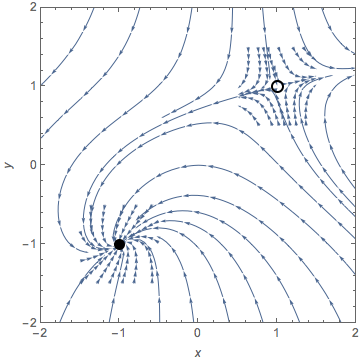
\includegraphics[width=3in]{img/Act19-02-20C08p1.png}

\end{questions}

\end{document}